\documentclass[tikz,border=5pt]{standalone}
\usepackage{tikz, amsmath}
\usetikzlibrary{arrows.meta, calc}

\begin{document}

%% ================================================================
%% Figure 1 – Levenberg–Marquardt: sparse geometric Jacobian J_V
%% ================================================================
%%
%% Front:  V0=(0,1.5) -- Va=(1.8,2.8) -- Vb=(4.3,2.2) -- V3=(6,3.5)
%% Va INSIDE cell (0,1), Vb INSIDE cell (2,1)  (no vertex on a grid face)
%% Normal at Va:
%%   seg V0->Va dir=(1.8,1.3), left-perp=(-1.3,1.8)/2.222=(-0.585,0.811)
%%   seg Va->Vb dir=(2.5,-0.6), left-perp=(0.6,2.5)/2.571=(0.233,0.972)
%%   avg(-0.352,1.783)/norm=(-0.193,0.981)
%% Displaced: Va'=(1.8-0.193*0.82, 2.8+0.981*0.82)=(1.642,3.605)
%%
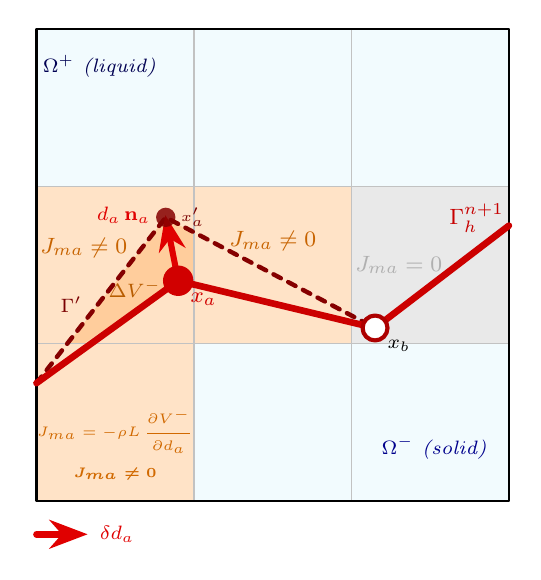
\begin{tikzpicture}[>=Stealth, font=\small, line cap=round, line join=round]

  %% ---- background + affected cells (orange) ----
  \fill[cyan!5]    (0,0) rectangle (6,6);
  \fill[orange!22] (0,0) rectangle (2,2);   %% J_ma != 0
  \fill[orange!22] (0,2) rectangle (2,4);   %% J_ma != 0
  \fill[orange!22] (2,2) rectangle (4,4);   %% J_ma != 0
  \fill[gray!17]   (4,2) rectangle (6,4);   %% J_ma = 0

  %% ---- swept volume DeltaV (between Gamma and Gamma') ----
  \begin{scope}
    \clip (0,0) rectangle (2,4);
    \fill[orange!55, opacity=0.50]
      (0.4,2.0) -- (0.6,2.0) -- (1.8,2.8) -- (2.0,2.7) -- (2.0,3.4) -- (1.642,3.605)-- cycle;
  \end{scope}
 

  %% ---- grid ----
  \draw[gray!48, thin] (0,0) grid[step=2] (6,6);
  \draw[black, thick] (0,0) rectangle (6,6);

  %% ---- displaced front Gamma' (dashed) ----
  \draw[red!52!black, dashed, line width=1.6pt]
    (0,1.5) -- (1.642,3.605) -- (4.3,2.2);
  \node[red!48!black, font=\scriptsize, anchor=east] at (0.70,2.5) {$\Gamma'$};

  %% ---- current front Gamma ----
  \draw[red!80!black, line width=2.4pt]
    (0,1.5) -- (1.8,2.8) -- (4.3,2.2) -- (6,3.5);
  \node[red!78!black, font=\footnotesize, right=2pt] at (5.05,3.60)
    {$\Gamma_h^{n+1}$};

  %% ---- normal displacement arrow:  n_a ~ (-0.193, 0.981), length 0.85 ----
  \draw[->, red!88!black, line width=2.2pt]
    (1.8,2.8) -- ++({-0.193*0.85},{0.981*0.85})
    node[left=1pt, font=\scriptsize] {$d_a\,\mathbf{n}_a$};

  %% ---- markers ----
  \fill[red!82!black] (1.8,2.8) circle (5.5pt);
  \node[below right=1pt, red!82!black, font=\footnotesize] at (1.8,2.8) {$x_a$};
  \fill[red!52!black, opacity=0.85] (1.642,3.605) circle (3.5pt);
  \node[right=2pt, red!48!black, font=\tiny] at (1.642,3.605) {$x_a'$};
  \fill[white] (4.3,2.2) circle (4.5pt);
  \draw[red!68!black, line width=1.5pt] (4.3,2.2) circle (4.5pt);
  \node[below right=1pt, font=\scriptsize] at (4.3,2.2) {$x_b$};

  %% ---- Jacobian entry labels ----
  \node[orange!82!black, font=\tiny, align=center] at (1.00,0.72)
    {$J_{ma} = -\rho L\,\dfrac{\partial V^-}{\partial d_a}$\\[4pt]
     $\boldsymbol{J_{ma} \neq 0}$};
  \node[orange!78!black, font=\footnotesize] at (0.6,3.22) {$J_{ma} \neq 0$};
  \node[orange!78!black, font=\footnotesize] at (3.00,3.3) {$J_{ma} \neq 0$};
  \node[gray!62,          font=\footnotesize] at (4.60,3.00) {$J_{ma} = 0$};

  %% ---- DeltaV label ----
  \node[orange!72!black, font=\scriptsize\itshape] at (1.25,2.70) {$\Delta V^-$};

  %% ---- phase labels ----
  \node[blue!55!black, font=\scriptsize\itshape] at (5.05,0.68) {$\Omega^-$ (solid)};
  \node[blue!32!black, font=\scriptsize\itshape] at (0.80,5.52) {$\Omega^+$ (liquid)};
  \draw[->, red!88!black, line width=2.4pt]    (0.0,-0.42) -- (0.65,-0.42);
  \node[right, font=\scriptsize, red!88!black]  at (0.68,-0.42)  {$\delta d_a$};
 

\end{tikzpicture}

\end{document}
